% SANCHARi -- editable two-column proceedings manuscript.
% The conference calls for 10-point, two-column Springer-style copy.
% Springer Nature's LNEE proceedings guide supplies the structure and
% reference conventions; its generic production template is not used here
% because the conference explicitly requests two columns.
\documentclass[10pt,a4paper,twocolumn]{article}
\usepackage[margin=2.2cm,top=2.0cm,bottom=2.1cm]{geometry}
\setlength{\columnsep}{0.62cm}
\usepackage[T1]{fontenc}
\usepackage[utf8]{inputenc}
\usepackage{lmodern}
\usepackage{microtype}
\usepackage{cite}
\usepackage{amsmath,amssymb,amsfonts}
\usepackage{graphicx}
\usepackage{textcomp}
\usepackage{booktabs}
\usepackage{tabularx}
\usepackage{multirow}
\usepackage[font=small,labelfont=bf]{caption}
\usepackage[hidelinks]{hyperref}
\setcounter{secnumdepth}{2}
\setlength{\parindent}{1em}
\setlength{\parskip}{0pt}
\pagestyle{empty}
\renewcommand{\refname}{References}
\renewcommand{\abstractname}{Abstract}

\begin{document}

\title{\bfseries\fontsize{14}{16}\selectfont SANCHARi: A Human-in-the-Loop Geospatial Framework for Satellite Road Network Extraction and Collaborative Curation}
\author{\small Ahmed Zyed K.A.\textsuperscript{1}, Alan Saji\textsuperscript{1}, Farhaan Nizam\textsuperscript{1},\\
\small Sreyas S Warrier\textsuperscript{1}, Shameem Ansar A\textsuperscript{1}, Suresh Francis\textsuperscript{2}\\[0.35em]
\footnotesize \textsuperscript{1}Department of Computer Science and Engineering, TKM College of Engineering, Kollam, Kerala, India\\
\footnotesize \textsuperscript{2}Kerala State Remote Sensing and Environment Centre, Vikas Bhavan, Thiruvananthapuram, Kerala, India\\
% REQUIRED BEFORE SUBMISSION: replace the following with the named corresponding author and real email.
\footnotesize Corresponding author: Ahmed Zyed K.A. (email to be supplied)}
\date{}

\maketitle

\begin{abstract}
Traditional geographic information systems are often built using centralized databases that do not account for rapid landscape changes and natural disasters. This paper proposes a crowdsourced, collaborative GIS with human-in-the-loop collaboration for generating and updating road information using an automated deep learning system, SANCHARi. An advanced U-Net++ architecture with an EfficientNet-B4 encoder is employed; the project reports approximately 80\% Intersection-over-Union for road segmentation on its DeepGlobe validation split. The paper further discusses a collaborative editing framework based on Next.js, Leaflet.js, and PostGIS for local administrators to review, edit, lock, and validate spatial vector graphics generated by the deep learning model. A 512-pixel overlapping inference scheme, four-way test-time augmentation, graph cleanup, and GeoJSON export connect the image model to the editor. The proposed workflow addresses challenges posed by canopy occlusion and the delay of automated map updates in diverse terrain. Kerala serves as the motivating application context and a qualitative system scenario; a separately labeled Kerala ground-truth test set and a measured collaborative-editor study remain future evaluation tasks.
\end{abstract}
\noindent\textbf{Keywords:} Collaborative GIS; deep learning; U-Net++; EfficientNet-B4; OpenStreetMap; WebGIS; participatory GIS.



\section{Introduction}
Accurate road and map networks are fundamental geospatial assets required to coordinate disaster response, and on a day-to-day basis, plan for better public administration. However, it becomes a bottleneck to consistently create and maintain such datasets, specifically in regions that frequently undergo dynamic environment changes.

\subsection{The Context of Kerala's Landscape}
Kerala's geophysical landscape is particularly challenging for accurate road mapping due to thick vegetation, canal systems, and seasonal flooding. Centralized mapping authorities can be slow to reflect changes on the ground, resulting in inevitably outdated information during emergency situations. 
\begin{itemize}
    \item \textbf{Canopy Occlusion:} Dense tropical vegetation and heavy tree plantations consistently tower over village roads and pathways, leading to automated models to completely miss out on detecting such features.
    \item \textbf{Hydrological Complexity:} The extensive networks of inland waterways and canals run parallel to these rural - and often urban - paths, or intersect them, which introduces a whole new layer of spectral ambiguity.
    \item \textbf{Dynamic Vulnerability:} Monsoon-driven floods destroy or temporarily realign crucial last-mile transport links overnight, creating life-and-death stakes for search-and-rescue teams.
\end{itemize}

\subsection{Research Question and Contributions}
The central question is how to turn a road probability map into a maintainable geographic network without treating an image classifier as the final cartographic authority. A useful system must preserve each candidate segment's geographic position and allow a knowledgeable reviewer to correct both omissions and false positives. The model supplies a draft, while the WebGIS maintains the editable spatial record. This distinction matters where an apparently continuous bright strip in an image may be a canal bank, roof edge, or temporary flood artifact.

This paper makes three connected contributions. First, it documents the implemented SANCHARi V4 path from overlapping satellite-image tiles through U-Net++ inference to a georeferenced road graph. Second, it specifies the editing and transaction path that places machine-produced vectors under human review. Third, it separates the reported DeepGlobe pixel-overlap result from the Kerala deployment motivation, so readers can identify what the available evidence establishes. The approach targets candidate generation and curation rather than a fully automatic authoritative road map.


\section{Literature Review}
The research pathway for road extraction as well as map maintenance divulges itself into two areas: The development and evolution of Collaborative WebGIS (online-based systems) as well as the current advancements in Deep Learning and its feature extraction techniques.

\subsection{Collaborative and Web-Based GIS Systems}
Collaborative GIS platforms have been improved for distributed urban planning and emergency management. Jing et al.~\cite{b1} proposed a version-based lightweight collaborative geospatial editing approach for urban planning management that used replication to achieve constraint-free editing. Butt et al.~\cite{b2} suggested GeoWebEX, an open-source online system for synchronous geospatial collaboration that enables users to share maps, conduct video and audio conferences, and make geo-referenced annotations in a web browser.

Moreover, cloud-based apps were also implemented for local management purposes. Kantartzis and Malesios~\cite{b3} suggested a decision support system (DSS) for forest road networks management that provided an open-source database of potential problem locations. Netek et al.~\cite{b4} assessed the use of cloud-based geospatial tools and revealed that GeOnline was the most appropriate such tool for executing process-driven operations directly in browsers. In addition, Pollino et al.~\cite{b5} employed open-source geospatial tools to design a conceptual model for managing probable damage caused by disastrous earthquakes. A separate collaborative high-definition mapping framework~\cite{b7} further illustrates how shared editing can be organized.

Table~\ref{tab:lit_review} contrasts representative editing and extraction systems with the integration considered here.

\begin{table*}[t]
\caption{Comparison of Collaborative GIS and Extraction Frameworks}
\begin{center}
\begin{tabularx}{\linewidth}{>{\hsize=0.6\hsize\raggedright\arraybackslash}X >{\hsize=1.2\hsize\raggedright\arraybackslash}X >{\hsize=1.2\hsize\raggedright\arraybackslash}X}
\toprule
\textbf{Study / System} & \textbf{Core Contribution} & \textbf{Limitations} \\
\midrule
Jing et al. (2019) & Developed a version-based lightweight collaborative GIS for urban planning. & Constrained by older, legacy desktop component systems (e.g., Delphi IDE). \\
\addlinespace
GeoWebEX (2018) & Open-source, browser-based synchronous collaboration with geo-referenced annotations. & Relies solely on manual human input; most effective only with GIS-experienced users. \\
\addlinespace
MAiD (2019) & Integrated machine learning into OpenStreetMap editor; increased mapping speeds by 3.5x. & Primarily designed to tackle the addition of major, arterial roads rather than complex rural trails. \\
\addlinespace
Sat2Graph (2020) & Uses Graph-tensor encoding (GTE) to extract network graphs directly, bypassing segmentation limits. & Purely automated framework lacking a human-in-the-loop collaborative editing interface. \\
\bottomrule
\end{tabularx}
\label{tab:lit_review}
\end{center}
\end{table*}

\subsection{Machine-Assisted Mapping and Automation}

The integration of machine learning into mapping workflows has drastically increased data generation speeds. Bastani et al.~\cite{b6} created a Machine-assisted iD (MAiD) -- an extension to the OpenStreetMap map editor that enables mappers to trace roads using machine assistance. The results show that in a Washington-area experiment, MAiD helped mappers to achieve 3.5x more roads traced than would otherwise be traced manually. Moreover, the number of traced roads exceeded hand-traced roads by 1.7x in a remote region of Indonesia. Shi et al.~\cite{b8} engineered a convolutional network based on GANs that reconstructs images with smoother appearance and better defined edges than those produced by standard segmentation procedures.

Recent research has been aimed at improving the topology of the generated results. Thus, Bastani et al.~\cite{b9} proposed RoadTracer -- an iterative search procedure that utilizes a CNN-based decision function to identify road junctions, yielding to 45\% more junctions than standard semantic segmentation approaches. He et al.~\cite{b10} proposed Sat2Graph, a framework that leverages a novel graph-tensor encoding to directly reconstruct road network graphs from satellite imagery, achieving the best performance across all topological similarity measures.

These studies address distinct outputs. Segmentation methods such as U-Net and U-Net++ predict occupied road pixels~\cite{b11,b13}; RoadTracer and Sat2Graph emphasize network connectivity~\cite{b9,b10}; collaborative systems emphasize the validity and provenance of edits~\cite{b1,b2,b6}. A high pixel IoU need not imply that a route is traversable: one missing bridge pixel can break an otherwise accurate network. Conversely, joining nearby but unrelated centerlines may improve visual continuity while creating an invalid turn. This paper combines pixel prediction, graph refinement, and an editor that can resolve ambiguous cases. The DeepGlobe challenge supplies the labeled image context for the reported segmentation comparison~\cite{b16}.


\section{Methodology}

\subsection{System Boundary and Data Flow}
The proposed system treats a predicted network as a versioned suggestion. An input coordinate or local image initiates inference; the service returns an EPSG:4326 GeoJSON FeatureCollection; the browser displays those candidates over imagery; and an authorized editor inspects, modifies, and commits selected geometries. A generated line is therefore distinct from an accepted road record. This separation lets automated coverage coexist with local knowledge about road status, seasonal passability, and mapping errors. The inference services and collaborative WebGIS are joined at the vector-data boundary, allowing their implementations to evolve independently.

Figure~\ref{fig:sanchari_pipeline} follows the model side of this boundary, and Fig.~\ref{fig:manual_editing_workflow} follows the curation side. The model repository provides the Python training and inference implementation. The interface screenshots and transaction description document the associated WebGIS design; they are not a quantified usability study.

The major novelty of this work resides in its peculiar integration of two separate geospatial paradigms: supervised deep-learning algorithms and participatory GIS (PGIS). Both fully automatic approaches and PGIS are well-established methods for generating standard vector data sets, but each has critical limitations, which, when used in isolation, significantly curtail their effectiveness in practice.

The major shortcoming of fully automatic approaches, implemented with convolutional neural networks, is the inability to deal with the complexities of real-world spatial data structures. In particular, deep-learning models in their current state cannot reliably process occlusions and are generally fairly brittle to variations in environmental conditions, leading to numerous erroneous lines in the generated output graphs, often resulting in fragmented outputs and machine hallucinations (confident, but wrong output from AI models). At the same time, PGIS - the fully manual paradigm of things - suffers from being extremely laborious, if not unrealistically demanding, in terms of the expertise required: only local administrative-level personnel can usually possess the domain knowledge necessary to digitize the vector data correctly.


The innovation of this project was to propose a concept of human-in-the-loop system that combined the strengths of both approaches while minimizing their weaknesses. This was achieved by designing the system around a dual-core design, which consisted of the following two interdependent components:
\begin{enumerate}
    \item \textbf{The Automated Bulk Vectorization Engine (SANCHARI):} A high-performance deep-learning backend tasked with the computationally heavy lifting of scanning vast expanses of satellite imagery to generate baseline candidate road geometries instantly.
    \item \textbf{The Collaborative Curation Interface (WebGIS):} A responsive, distributed frontend platform that ingests the machine-generated vectors and empowers local administrative experts to provide critical ``last-mile'' spatial validation.
\end{enumerate}

These two elements are designed to share a geospatial database through an API, allowing edits to be synchronized and providing overall coherence. In effect, the proposed system can rapidly generate an initial set of candidate road lines and allow authorized local government experts and administrators to edit the automatically generated geometry while viewing changes in the web interface. Human curators can remove inauthentic lines while retaining authentic model suggestions. The expected acceleration over purely manual digitization is a hypothesis to test with the reviewer-time protocol in Sect.~\ref{sec:field_protocol}.

% ---------------------------------------------------------------------------
\subsection{Automated Deep Learning Pipeline (SANCHARI Model)}
% ---------------------------------------------------------------------------

The SANCHARI model is an end-to-end pipeline that accepts a geographic
coordinate or a local GeoTIFF file and returns a georeferenced GeoJSON
FeatureCollection of road polylines. The pipeline is illustrated in
Fig.~\ref{fig:sanchari_pipeline}.

\begin{figure*}[t]
\centering
\fbox{\parbox[c][1.0cm][c]{2.2cm}{\centering\footnotesize Coordinate or\\GeoTIFF imagery}}\hspace{0.15cm}$\longrightarrow$\hspace{0.15cm}
\fbox{\parbox[c][1.0cm][c]{2.2cm}{\centering\footnotesize 512-pixel tiles\\and four-way TTA}}\hspace{0.15cm}$\longrightarrow$\hspace{0.15cm}
\fbox{\parbox[c][1.0cm][c]{2.2cm}{\centering\footnotesize U-Net++ /\\EfficientNet-B4}}\hspace{0.15cm}$\longrightarrow$\hspace{0.15cm}
\fbox{\parbox[c][1.0cm][c]{2.2cm}{\centering\footnotesize Probability mask\\and graph cleanup}}\hspace{0.15cm}$\longrightarrow$\hspace{0.15cm}
\fbox{\parbox[c][1.0cm][c]{2.2cm}{\centering\footnotesize EPSG:4326\\GeoJSON roads}}
\caption{The end-to-end SANCHARi V4 architecture pipeline, from imagery acquisition to GeoJSON road-network vectorization.}
\label{fig:sanchari_pipeline}
\end{figure*}

\subsubsection{Model Architecture}

The V4 model employs a \textbf{U-Net++} decoder~\cite{b13} with an
\textbf{EfficientNet-B4} encoder~\cite{b14} pretrained on ImageNet. U-Net++
replaces the standard single skip connection per depth level with
dense nested sub-networks that aggregate features across all encoder
scales, closing the semantic gap and preserving thin, single-pixel-wide
road centrelines. EfficientNet-B4 uses compound scaling to jointly
optimise network depth, width, and resolution, yielding richer texture
discrimination than the ResNet34 backbone~\cite{b12} used in earlier versions.

\paragraph{Training Data and Split.}
The implementation preprocesses paired DeepGlobe satellite JPEG images and road-mask PNG files~\cite{b16}. Its preprocessing script reflect-pads each source image as needed, then extracts $512\times512$ image-mask tiles at a 256-pixel stride. Only the first three image bands are retained, and grayscale mask values greater than 127 are interpreted as road. The training script sorts the resulting tile names and uses a random 85\%/15\% tile-level training-validation split with seed 42. This is an important qualification: neighboring overlapping tiles can enter different partitions, so the reported validation result should not be interpreted as performance on entirely unseen geographic scenes. A source-image or geographic-region split is needed for a stronger estimate of transfer to Kerala.

The data loader normalizes RGB values with ImageNet channel means $(0.485,0.456,0.406)$ and standard deviations $(0.229,0.224,0.225)$. Training-only augmentation includes flips, rotations, transpose, grid distortion, elastic deformation, brightness and color changes, gamma variation, Gaussian noise, and blur. Masks undergo corresponding spatial transforms but not photometric transforms. Validation uses normalization without stochastic augmentation. These operations increase the range of appearances seen during training; they do not by themselves demonstrate robustness to cloud, floodwater, or a different sensor.

\subsubsection{Training Strategy}

Road extraction is a heavily class-imbalanced binary segmentation task.
The V4 training procedure is organized as up to three sequential phases.

\textbf{Phase 1 --- Combo Loss.} The primary loss combines Dice Loss
and Focal Loss in equal proportion:
\begin{equation}
\mathcal{L}_{\text{Combo}} = 0.5 \cdot \mathcal{L}_{\text{Dice}}
                            + 0.5 \cdot \mathcal{L}_{\text{Focal}}
\label{eq:combo}
\end{equation}
Dice Loss optimises pixel-level overlap and handles class imbalance;
Focal Loss down-weights easy background pixels and forces the model to
focus on hard examples such as road edges obscured by shadows and
canopy.

The main training configuration uses AdamW at a starting learning rate of $5\times10^{-4}$, weight decay $10^{-4}$, cosine annealing over 50 epochs, minibatches of eight, and two-step gradient accumulation. The nominal effective batch size is therefore 16 for complete accumulation pairs. Checkpoints are selected using validation IoU. The implementation calculates IoU after a 0.5 probability threshold during validation, whereas the default exported-map threshold is 0.45; these thresholds refer to different stages and should be reported separately.

\textbf{Phase 2 --- Hard Negative Mining.} After main training, the
bottom 20\% of training samples by per-image IoU are identified and
the model is fine-tuned exclusively on these hard examples, improving
performance on deeply occluded intersections and canopy-covered roads.

\textbf{Phase 3 --- Lov\'{a}sz Fine-Tuning.} A final fine-tuning phase
replaces the loss with the Lov\'{a}sz-Softmax loss~\cite{b15}, which
provides a convex surrogation of the Jaccard index and directly
optimises the reported IoU metric rather than a differentiable
approximation of it.

The hard-sample phase is optional in the training script and runs for ten additional epochs at $10^{-5}$ when enabled. Lov\'{a}sz fine-tuning is a separate script initialized from saved V4 weights and configured for 20 epochs at $10^{-5}$. The project guide describes these as a three-stage strategy, but does not provide separate validation scores for each stage. Consequently, the version table below is a historical summary, not an ablation proving the effect of any single choice. A controlled ablation would hold the data split, seed, and threshold fixed while changing one component at a time.

\subsubsection{Inference and Post-Processing}

During inference, input imagery is decomposed into $512 \times 512$
patches with 50\% overlap. Each patch is processed with \textbf{4-way
Test Time Augmentation} (original, horizontal flip, vertical flip,
$90^{\circ}$ rotation), and the four resulting probability maps are
averaged before being stitched back into a full-image probability map.

The raw probability map is then refined by a \textbf{graph-theoretic
post-processing} pipeline rather than simple morphological dilation,
which would destroy road topology. The pipeline thresholds the
probability map, fills small holes, uses a KD-tree over skeleton
endpoints to close small gaps, skeletonises the binary mask to a
1-pixel-wide centreline, and converts the skeleton into a NetworkX
graph via \texttt{sknw}. Iterative graph pruning then removes short
dead-end spurs, false self-loops, and redundant parallel edges. The
cleaned graph is finally vectorised and exported as an EPSG:4326
GeoJSON FeatureCollection.

\paragraph{From Pixel Coordinates to Geography.}
The implementation applies the raster window's affine transform to graph-edge pixel coordinates, simplifies the resulting lines in the source projected coordinate system, and reprojects them to WGS84 for GeoJSON export. A missing or mismatched affine transform would shift otherwise plausible roads away from the imagery; coordinate-reference-system conversion is part of the output contract rather than a display detail. The code stores cleaned road segments as a MultiLineString within a FeatureCollection. Its simplification parameters are heuristic and may remove small bends or short links where pixel scale differs from the assumed projection.

The 0.45 threshold initiates mask cleanup. The current implementation fills holes smaller than 400 pixels, connects skeleton endpoints within a 25-pixel search radius, removes small objects, applies a disk-radius-three closing operation, and skeletonizes the cleaned mask. It then builds a multigraph and prunes short terminal spurs, loops, and redundant parallel edges. Gap closing is distance based and does not test road orientation or image evidence between endpoints; a reviewer remains necessary where nearby endpoints belong to different streets. Pixel-distance rules also change their ground-distance meaning when input resolution changes.

\subsubsection{Deployment}

Two Dockerised FastAPI services expose the pipeline: a \textbf{GEE
API} (port 8001) that fetches live NAIP or Sentinel-2 imagery via the
Google Earth Engine API, and a \textbf{Local GeoTIFF API} (port 8000)
that operates entirely offline against user-supplied \texttt{.tif}
files.

The Earth Engine mode requests imagery for a coordinate using collection and date filters. NAIP is a United States source; Sentinel-2 has broader coverage at a coarser native resolution. Neither source can be assumed to show a newly changed road until an appropriately dated, sufficiently clear scene is available. The local mode searches files covering the coordinate, transforms WGS84 into the raster's native coordinate system, reads a centered $1024\times1024$ window, and runs the same patch inference and vectorization path. Both services return candidate road geometry, not a validated route layer.

\begin{table}[htbp]
\caption{System Technology Stack}
\begin{center}
\small
\begin{tabularx}{\linewidth}{>{\hsize=0.6\hsize\raggedright\arraybackslash}X >{\hsize=1.4\hsize\raggedright\arraybackslash}X}
\toprule
\textbf{Layer / Domain} & \textbf{Technologies} \\
\midrule
Model Architecture & PyTorch, \texttt{segmentation\_models\_pytorch}, \texttt{timm} \\
\addlinespace
Augmentation & Albumentations (\texttt{GridDistortion}, \texttt{ElasticTransform}) \\
\addlinespace
Spatial Data & \texttt{rasterio}, \texttt{pyproj}, GeoPandas \\
\addlinespace
Graph \& Topology & \texttt{sknw}, NetworkX, Shapely, \texttt{scikit-image} \\
\addlinespace
Satellite Imagery & Google Earth Engine API (NAIP / Sentinel-2) \\
\addlinespace
API Services & FastAPI, Uvicorn, Pydantic \\
\addlinespace
Frontend WebGIS & Next.js, React.js, Leaflet.js \\
\addlinespace
Backend \& Database & Node.js, Express.js, PostgreSQL/PostGIS, GeoServer \\
\addlinespace
Deployment & Docker, docker-compose (GPU-optional) \\
\bottomrule
\end{tabularx}
\label{tab:tech_stack}
\end{center}
\end{table}


\subsection{Collaborative Web Architecture}
Table~\ref{tab:tech_stack} lists the implementation layers that connect model inference, geospatial processing, and the editor.
To harness human-enabled context and knowledge about the existing pipeline that the model cannot replicate, this system incorporates a WebGIS architecture to facilitate interactive and collaborative road-network editing, as illustrated in Fig. \ref{fig:manual_editing_workflow}.

The browser and model service exchange geometries through GeoJSON in WGS84. The editing stack uses Leaflet to visualize and change candidate features, Turf.js to split or subtract geometry, GeoServer to expose geospatial layers and receive transactions, and PostGIS to persist accepted changes. The interaction is intentionally staged: inspect the source imagery, select a candidate or draw an omitted segment, validate the edit, then commit it. A candidate should retain a review state and provenance so that a later operator can distinguish machine output from an approved correction. This is a design requirement for operational use, not a measured claim about the present screenshots.

\begin{itemize}
    \item \textbf{Frontend Layer \& Map Initialization:} The user interface leverages Leaflet.js and Leaflet.draw to support interactive editing of vector data. Upon loading, the map retrieves FlatGeobuf data through HTTP range requests from GeoServer, using a client-side spatial index to speed up data parsing. When a user selects a region, the system uses the area's bounding box to query relevant features, which are then transformed into an in-memory GeoJSON (RFC 7946) copy for editing.
    \item \textbf{Client-Side Geometry Processing:} For efficient handling of manual edits, Turf.js acts as the geometry processing engine on the client. Users can either draw LineStrings freehand to add new roads or create polygons to remove existing segments. During deletion operations, functions such as \texttt{turf.lineSplit()} and \texttt{turf.difference()} are used to split roads at the boundary of the erase area, distinguishing segments to retain from those to remove. All edited geometries are checked for self-intersections before being finalized.
    \item \textbf{Transaction, Sync, and Database:} Synchronization is managed through OGC WFS-T (Web Feature Service -- Transactional). Edits made during a session are grouped and formatted into a WFS-T-compliant XML payload, with GeoJSON features converted to GML to represent insertions, updates, and deletions. This payload is sent via HTTP POST to GeoServer, which translates the request into SQL commands executed on the PostGIS database. Changes are applied atomically, and the response---parsed from the returned XML---provides confirmation of the transaction (number of features inserted, updated, deleted) before the updated map view is refreshed in the interface.
\end{itemize}

\paragraph{Editing Invariants and Review.}
Insertion, deletion, and modification have different effects on network connectivity. A drawn LineString must snap or be explicitly joined to the intended network nodes before it can repair a routing gap. An erase polygon should remove only the intersected parts of a selected line, leaving the retained segments as valid geometries. A moved vertex can create a self-intersection or an unintended junction even if the feature remains syntactically valid GeoJSON. Therefore the review step should check geometry validity, local topology, imagery alignment, and the editor's reason for each change. The change log can support rollback and provenance, but its existence alone does not establish audit completeness or conflict-free simultaneous editing. Concurrent edit semantics require explicit lock or version checks to prevent a late transaction from overwriting another reviewer.

\begin{figure*}[t]
\centering
\fbox{\parbox[c][1.0cm][c]{2.2cm}{\centering\footnotesize Load map and\\candidate roads}}\hspace{0.15cm}$\longrightarrow$\hspace{0.15cm}
\fbox{\parbox[c][1.0cm][c]{2.2cm}{\centering\footnotesize Select area and\\review in Leaflet}}\hspace{0.15cm}$\longrightarrow$\hspace{0.15cm}
\fbox{\parbox[c][1.0cm][c]{2.2cm}{\centering\footnotesize Draw, split, or\\erase using Turf.js}}\hspace{0.15cm}$\longrightarrow$\hspace{0.15cm}
\fbox{\parbox[c][1.0cm][c]{2.2cm}{\centering\footnotesize Commit WFS-T\\to PostGIS}}\hspace{0.15cm}$\longrightarrow$\hspace{0.15cm}
\fbox{\parbox[c][1.0cm][c]{2.2cm}{\centering\footnotesize Refresh map\\and change log}}
\caption{The SANCHARi manual editing workflow, detailing map preparation, geometry editing, and GeoServer WFS-T synchronization.}
\label{fig:manual_editing_workflow}
\end{figure*}

\subsection{Reproducibility and Error Tracing}
The implementation can be replayed from a fixed input image or coordinate, a chosen model checkpoint, and a post-processing configuration. For a reproducible prediction, the recorded input should include the imagery collection or GeoTIFF identifier, acquisition date where available, raster resolution, crop bounds, native coordinate system, and model-weight version. The output should retain the probability map, thresholded mask, skeleton, graph, and final GeoJSON. These intermediate artifacts make it possible to locate an error in image acquisition, pixel prediction, graph cleanup, or coordinate conversion, instead of attributing every cartographic defect to the neural network.

The two API modes have different repeatability constraints. A local GeoTIFF window is stable as long as the file and coordinate are unchanged. An Earth Engine query can select a different scene as a collection updates or filtering rules change; its date and image identifier therefore need to be stored with the result. Repeated predictions should also log the 0.45 map threshold and graph-cleanup distances. If a candidate line is manually corrected, its edit history should identify the source prediction and the accepted geometry. This chain of provenance supports later review when imagery is replaced or a road's condition changes.

These are reproducibility requirements for a rigorous deployment. The present repository contains the model scripts, trained V4 weights, and saved inference examples, but the materials supplied with this paper do not include a frozen experiment manifest linking every reported historical IoU value to a checkpoint and scene list. The paper therefore reports those values at the precision supported by the project documentation and treats cross-version comparisons as descriptive.

\section{Results and Discussions}

\subsection{Evaluation Scope and Metric}
The numerical IoU values in Table~\ref{tab:model_evol} are reported in the project guide and original draft. For a binary predicted road mask $P$ and labeled mask $G$, IoU is $|P\cap G|/|P\cup G|$. It measures overlap of road pixels and is sensitive to threshold choice and label width. The training code computes validation IoU on minibatches after sigmoid and a 0.5 threshold, then averages those batch values; the post-processing service uses 0.45 for candidate generation. The paper does not have a released per-image prediction ledger, confidence intervals, or an independent Kerala ground-truth set. The values are thus presented as project-reported validation results, not as a new independent benchmark or a quantified measure of collaborative mapping quality.

An end-to-end evaluation should additionally measure road-graph connectivity, false intersections, path-length error, reviewer time, and edit acceptance rate. These quantities answer different questions from pixel IoU. For example, an isolated false-positive service road may have little effect on total pixel overlap but create a consequential routing error; reconnecting one obscured bridge may barely change IoU while restoring access to an entire neighborhood. Such outcomes motivate the human review layer, but they have not yet been quantified for the case-study regions.

\subsection{Empirical Case Study Regions}
The original project draft identifies heterogeneous pilot contexts in Kerala for qualitative system assessment. They motivate targeted validation, but the available project material does not include a labeled Kerala sample count or a separate Kerala IoU calculation.

\begin{itemize}
    \item \textbf{Zone A (Melila Panchayat):} Dense multi-tier canopy cover, narrow unpaved tracks, requiring high model sensitivity and local human validation to connect obscured segments.
    \item \textbf{Zone B (Urban Core):} High impervious surface ratios and concrete infrastructures that spectrally mimic road corridors.
    \item \textbf{Zone C (Coastal Region):} High-reflectance sandy soils and roads running parallel to backwaters, testing the model's spatial context awareness.
\end{itemize}

\subsection{Model Evolution and Performance}
The automated extraction model evolved significantly to address the cartographic demands of the study regions. 

\begin{table*}[t]
\caption{Project-Reported Model Evolution and Approximate Validation IoU}
\begin{center}
\begin{tabularx}{\linewidth}{>{\hsize=0.4\hsize\raggedright\arraybackslash}X >{\hsize=1.2\hsize\raggedright\arraybackslash}X >{\hsize=0.4\hsize\raggedright\arraybackslash}X}
\toprule
\textbf{Version} & \textbf{Architecture Changes} & \textbf{Validation IoU} \\
\midrule
V1 & Custom U-Net (scratch), BCE Loss & 54\% - 55\% \\
\addlinespace
V2 & ResNet34 Encoder, Dice Loss & 62.8\% - 68\% \\
\addlinespace
V3 & Sliding Window TTA, Attention Gates & 75\% \\
\addlinespace
V4 & EfficientNet-B4, U-Net++, Combo/Lov\'{a}sz Loss, Graph Pruning & 80\% \\
\bottomrule
\end{tabularx}
\label{tab:model_evol}
\end{center}
\end{table*}

The V1 baseline custom U-Net struggled severely with connectivity, with a reported IoU of approximately 54\%. Transitioning to a pre-trained ResNet34 backbone (V2) raised the reported IoU to 62.8\%. The V4 pipeline, utilizing the EfficientNet-B4 backbone and graph-theoretic post-processing suite, is reported at approximately 80\% on the DeepGlobe validation tiles. The draft describes fewer false positives from shadows and parking lots after GridDistortion augmentation and four-way test-time augmentation (TTA), but does not provide a controlled count for Zone B. Figure~\ref{fig:example_output} shows one saved inference output to illustrate the candidate overlay without treating it as a labeled accuracy test.

\begin{figure*}[t]
\centering
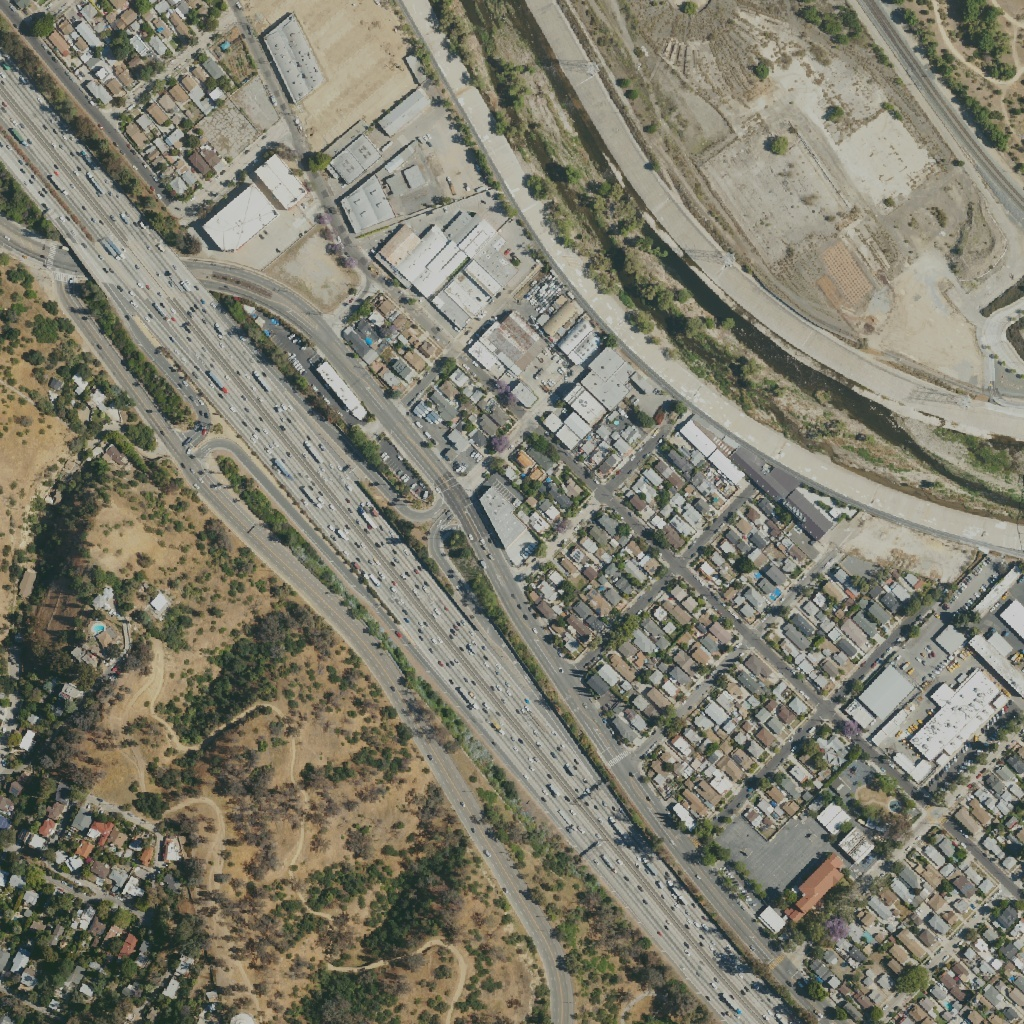
\includegraphics[width=0.46\textwidth]{example-road-input.jpg}\hfill
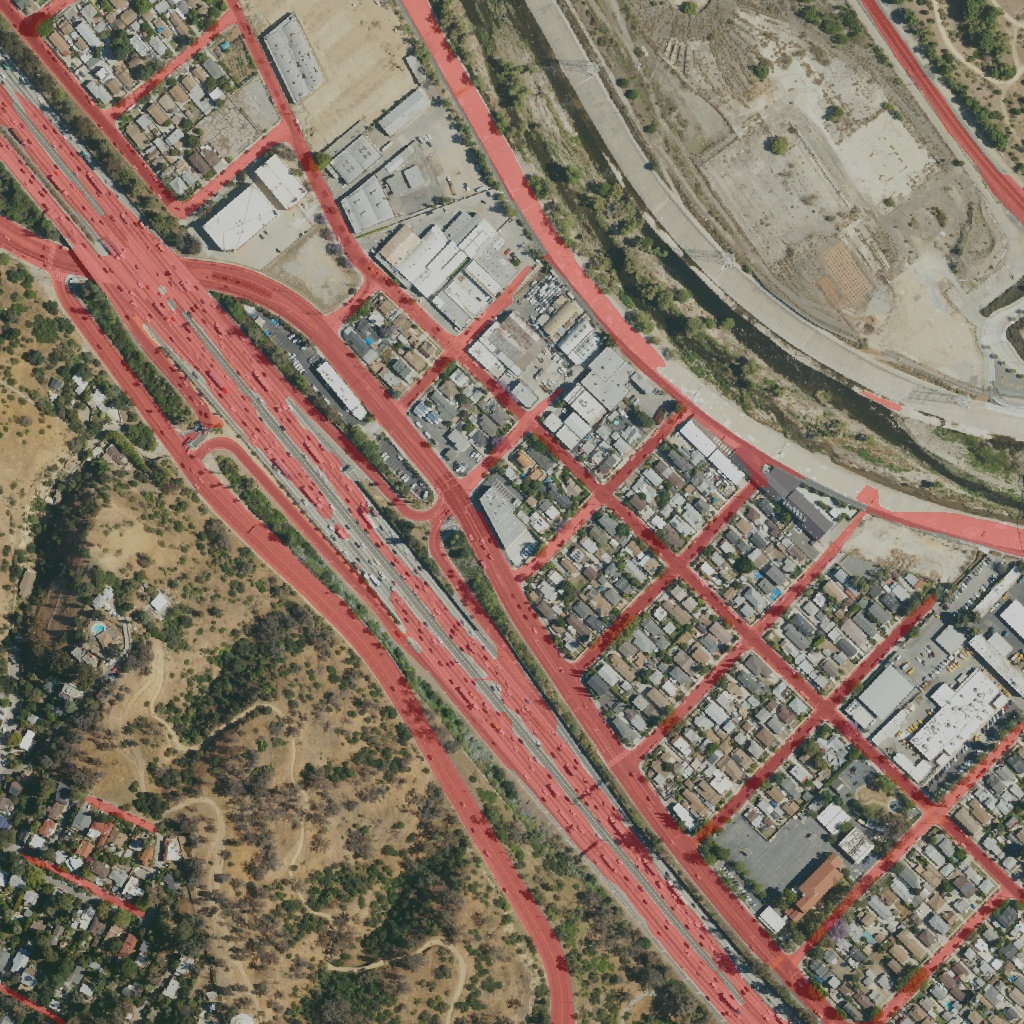
\includegraphics[width=0.46\textwidth]{example-road-overlay.jpg}
\caption{Illustrative saved inference output from the model repository for an NAIP scene near Los Angeles, California: input image (left) and candidate-road overlay (right). The image has no accompanying reference mask in this paper; it demonstrates output form, not Kerala accuracy.}
\label{fig:example_output}
\end{figure*}

\subsection{System Interface and Usability}
Despite the reported 80\% validation IoU, canopy occlusion in Zone A (Melila) is expected to introduce disconnects that need local review. The collaborative web application provides the intended intervention path.

% Placeholder for Home Page Screenshot
\begin{figure}[htbp]
\centerline{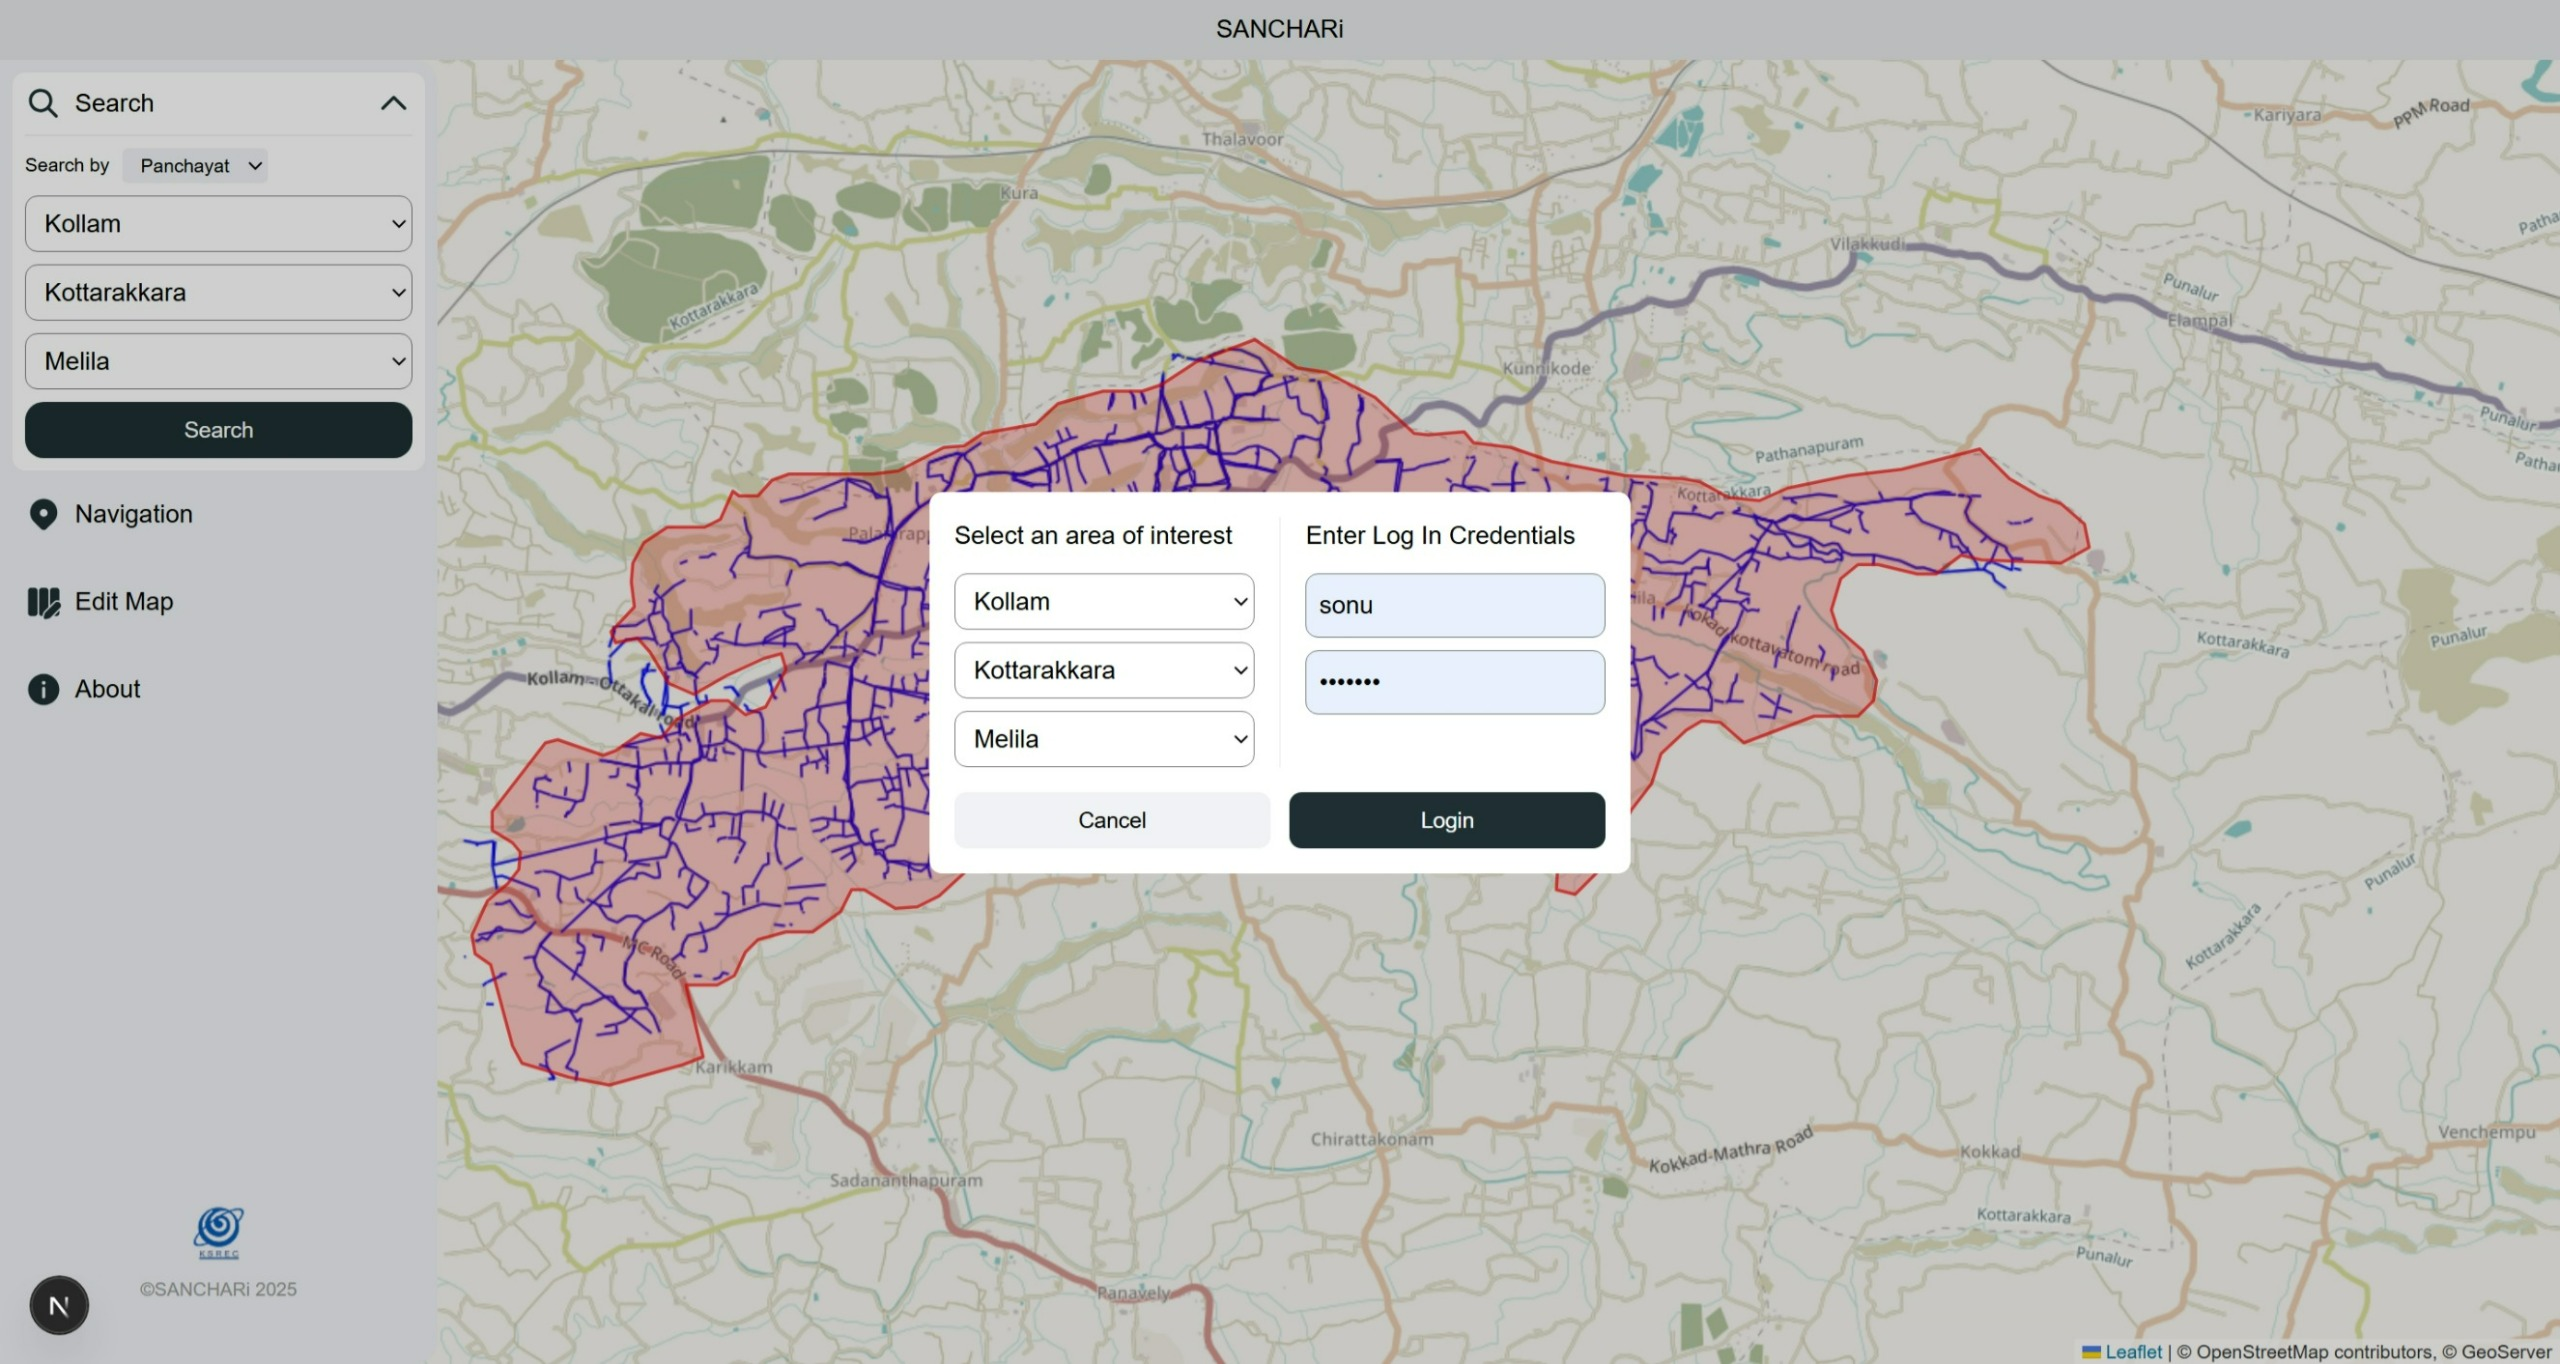
\includegraphics[width=0.9\linewidth]{homepage.jpg}}
\caption{Home Page Interface locked at Kollam city, demonstrating hierarchical navigation and search tools for local Panchayat administration.}
\label{fig:homepage}
\end{figure}

% Placeholder for Sidebar and Editing Tools Screenshot
\begin{figure}[htbp]
\centerline{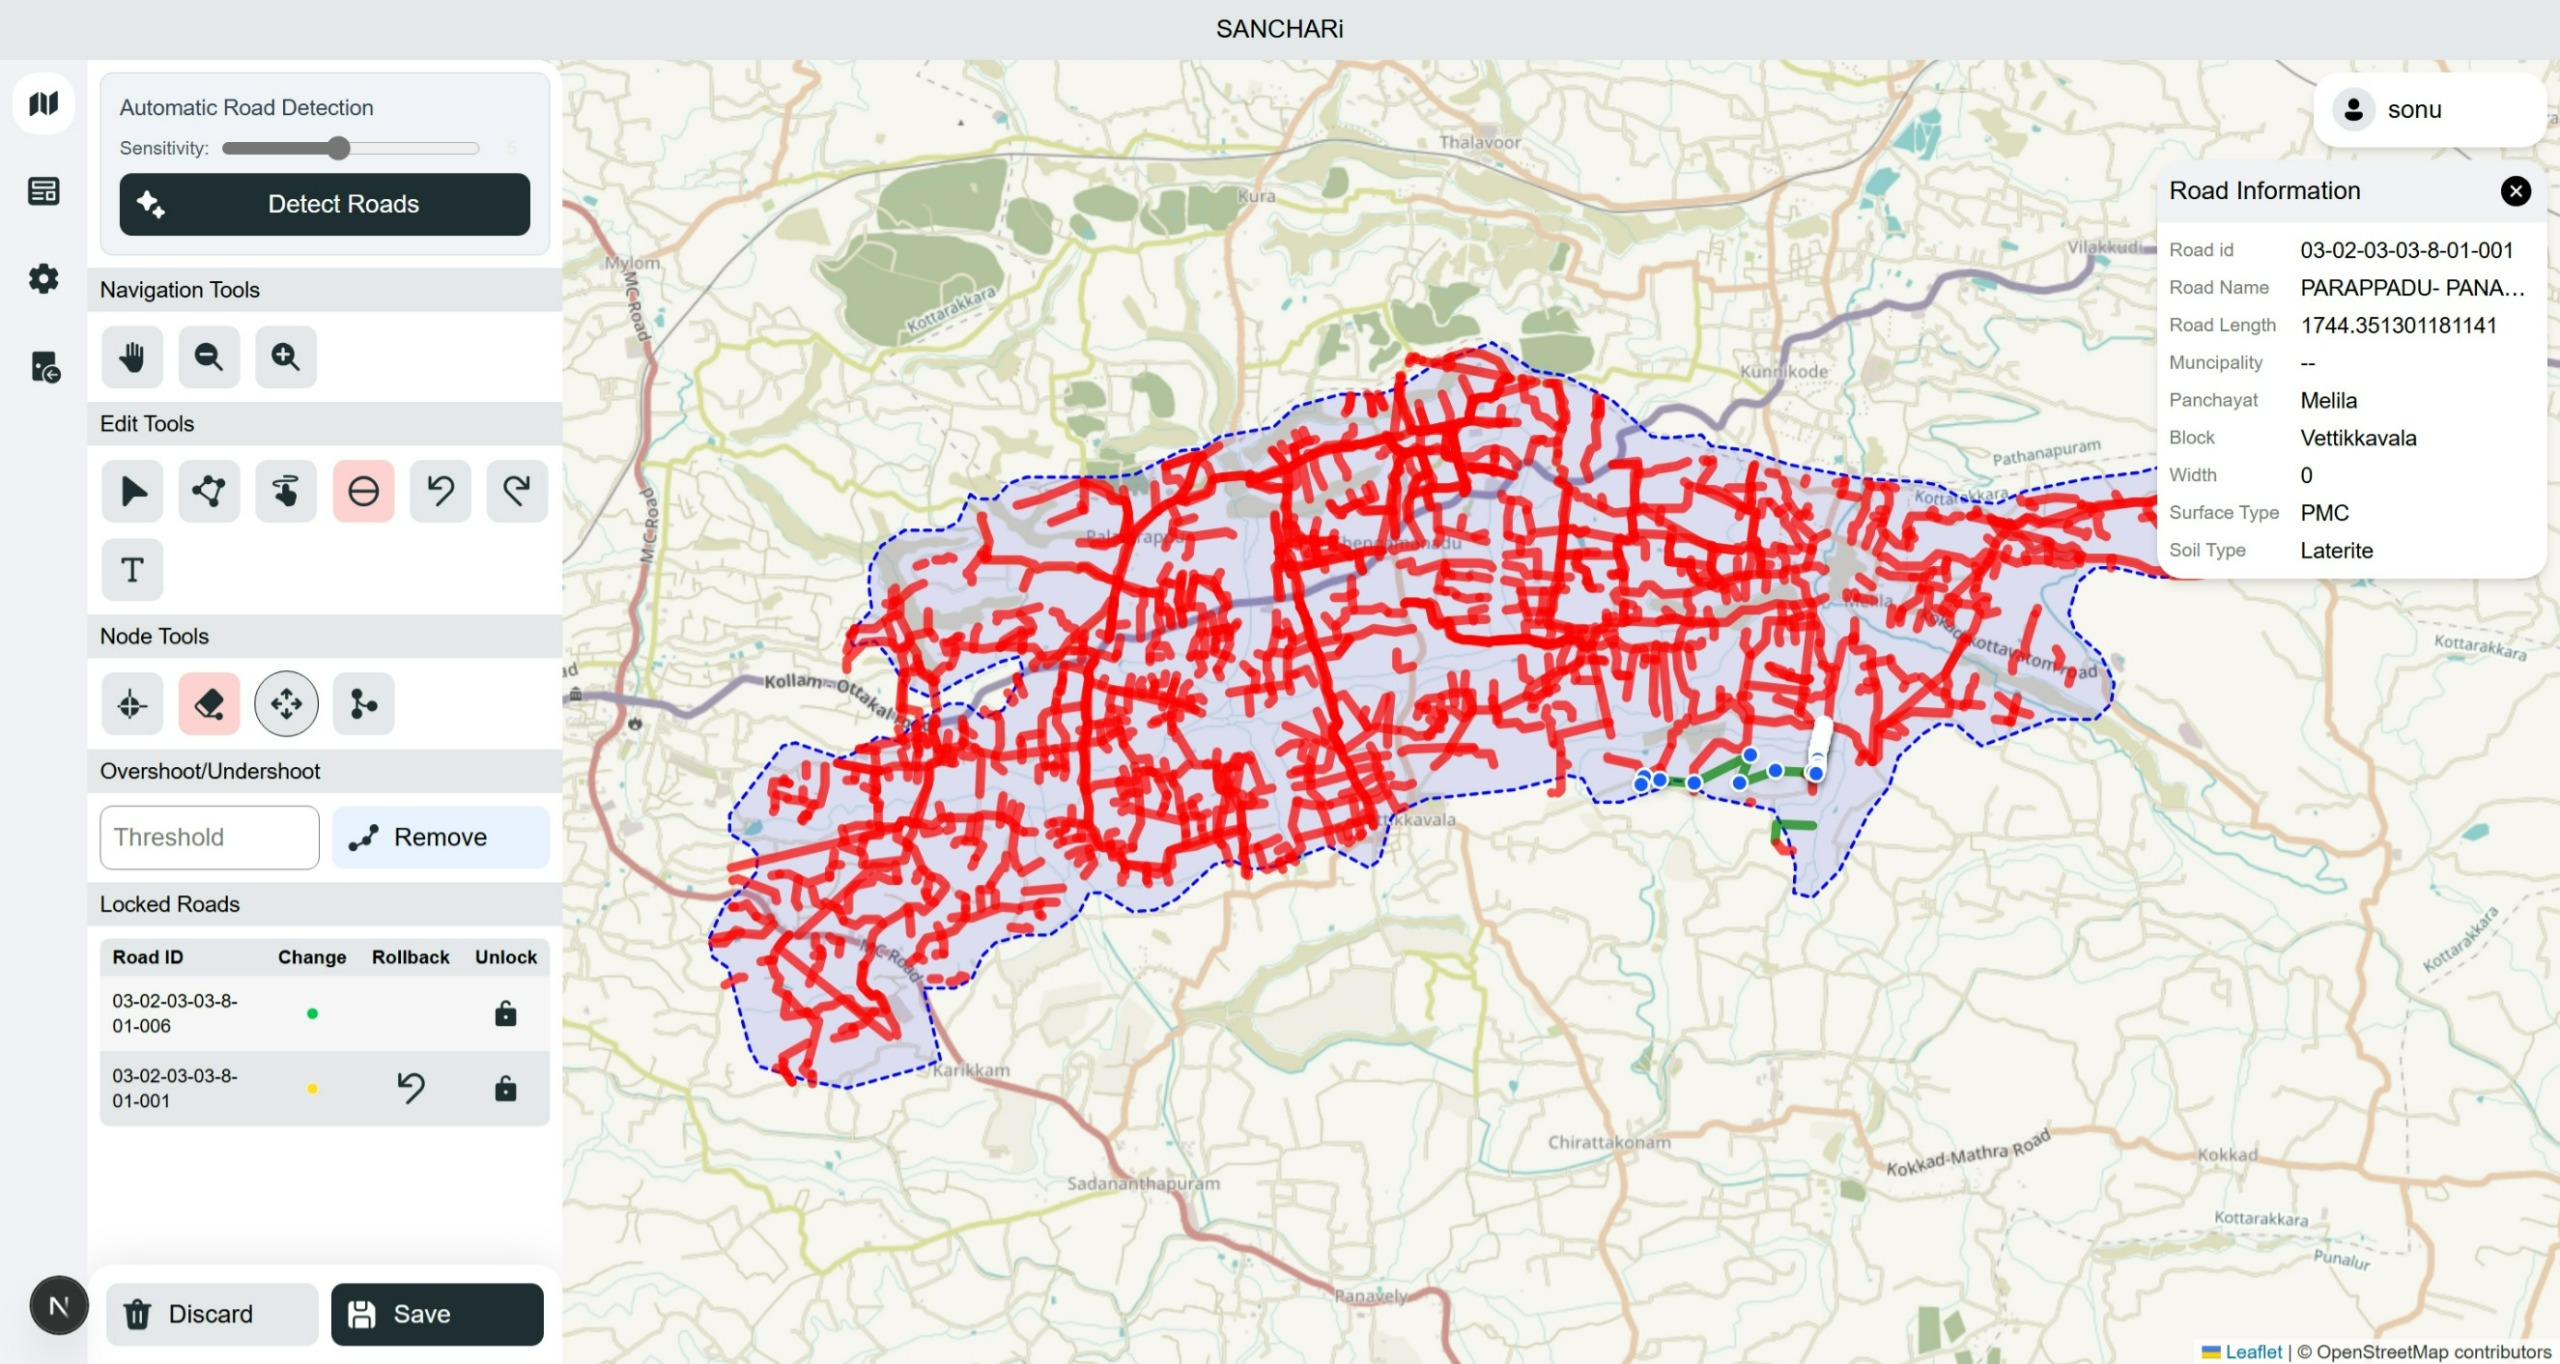
\includegraphics[width=0.9\linewidth]{sidebar.jpg}}
\caption{Sidebar functionalities displaying automated road detection triggers, Leaflet-powered node editing tools, and topological overshoot/undershoot correction limits.}
\label{fig:sidebar}
\end{figure}

% Placeholder for Road Selection and Change Log Screenshot
\begin{figure}[htbp]
\centerline{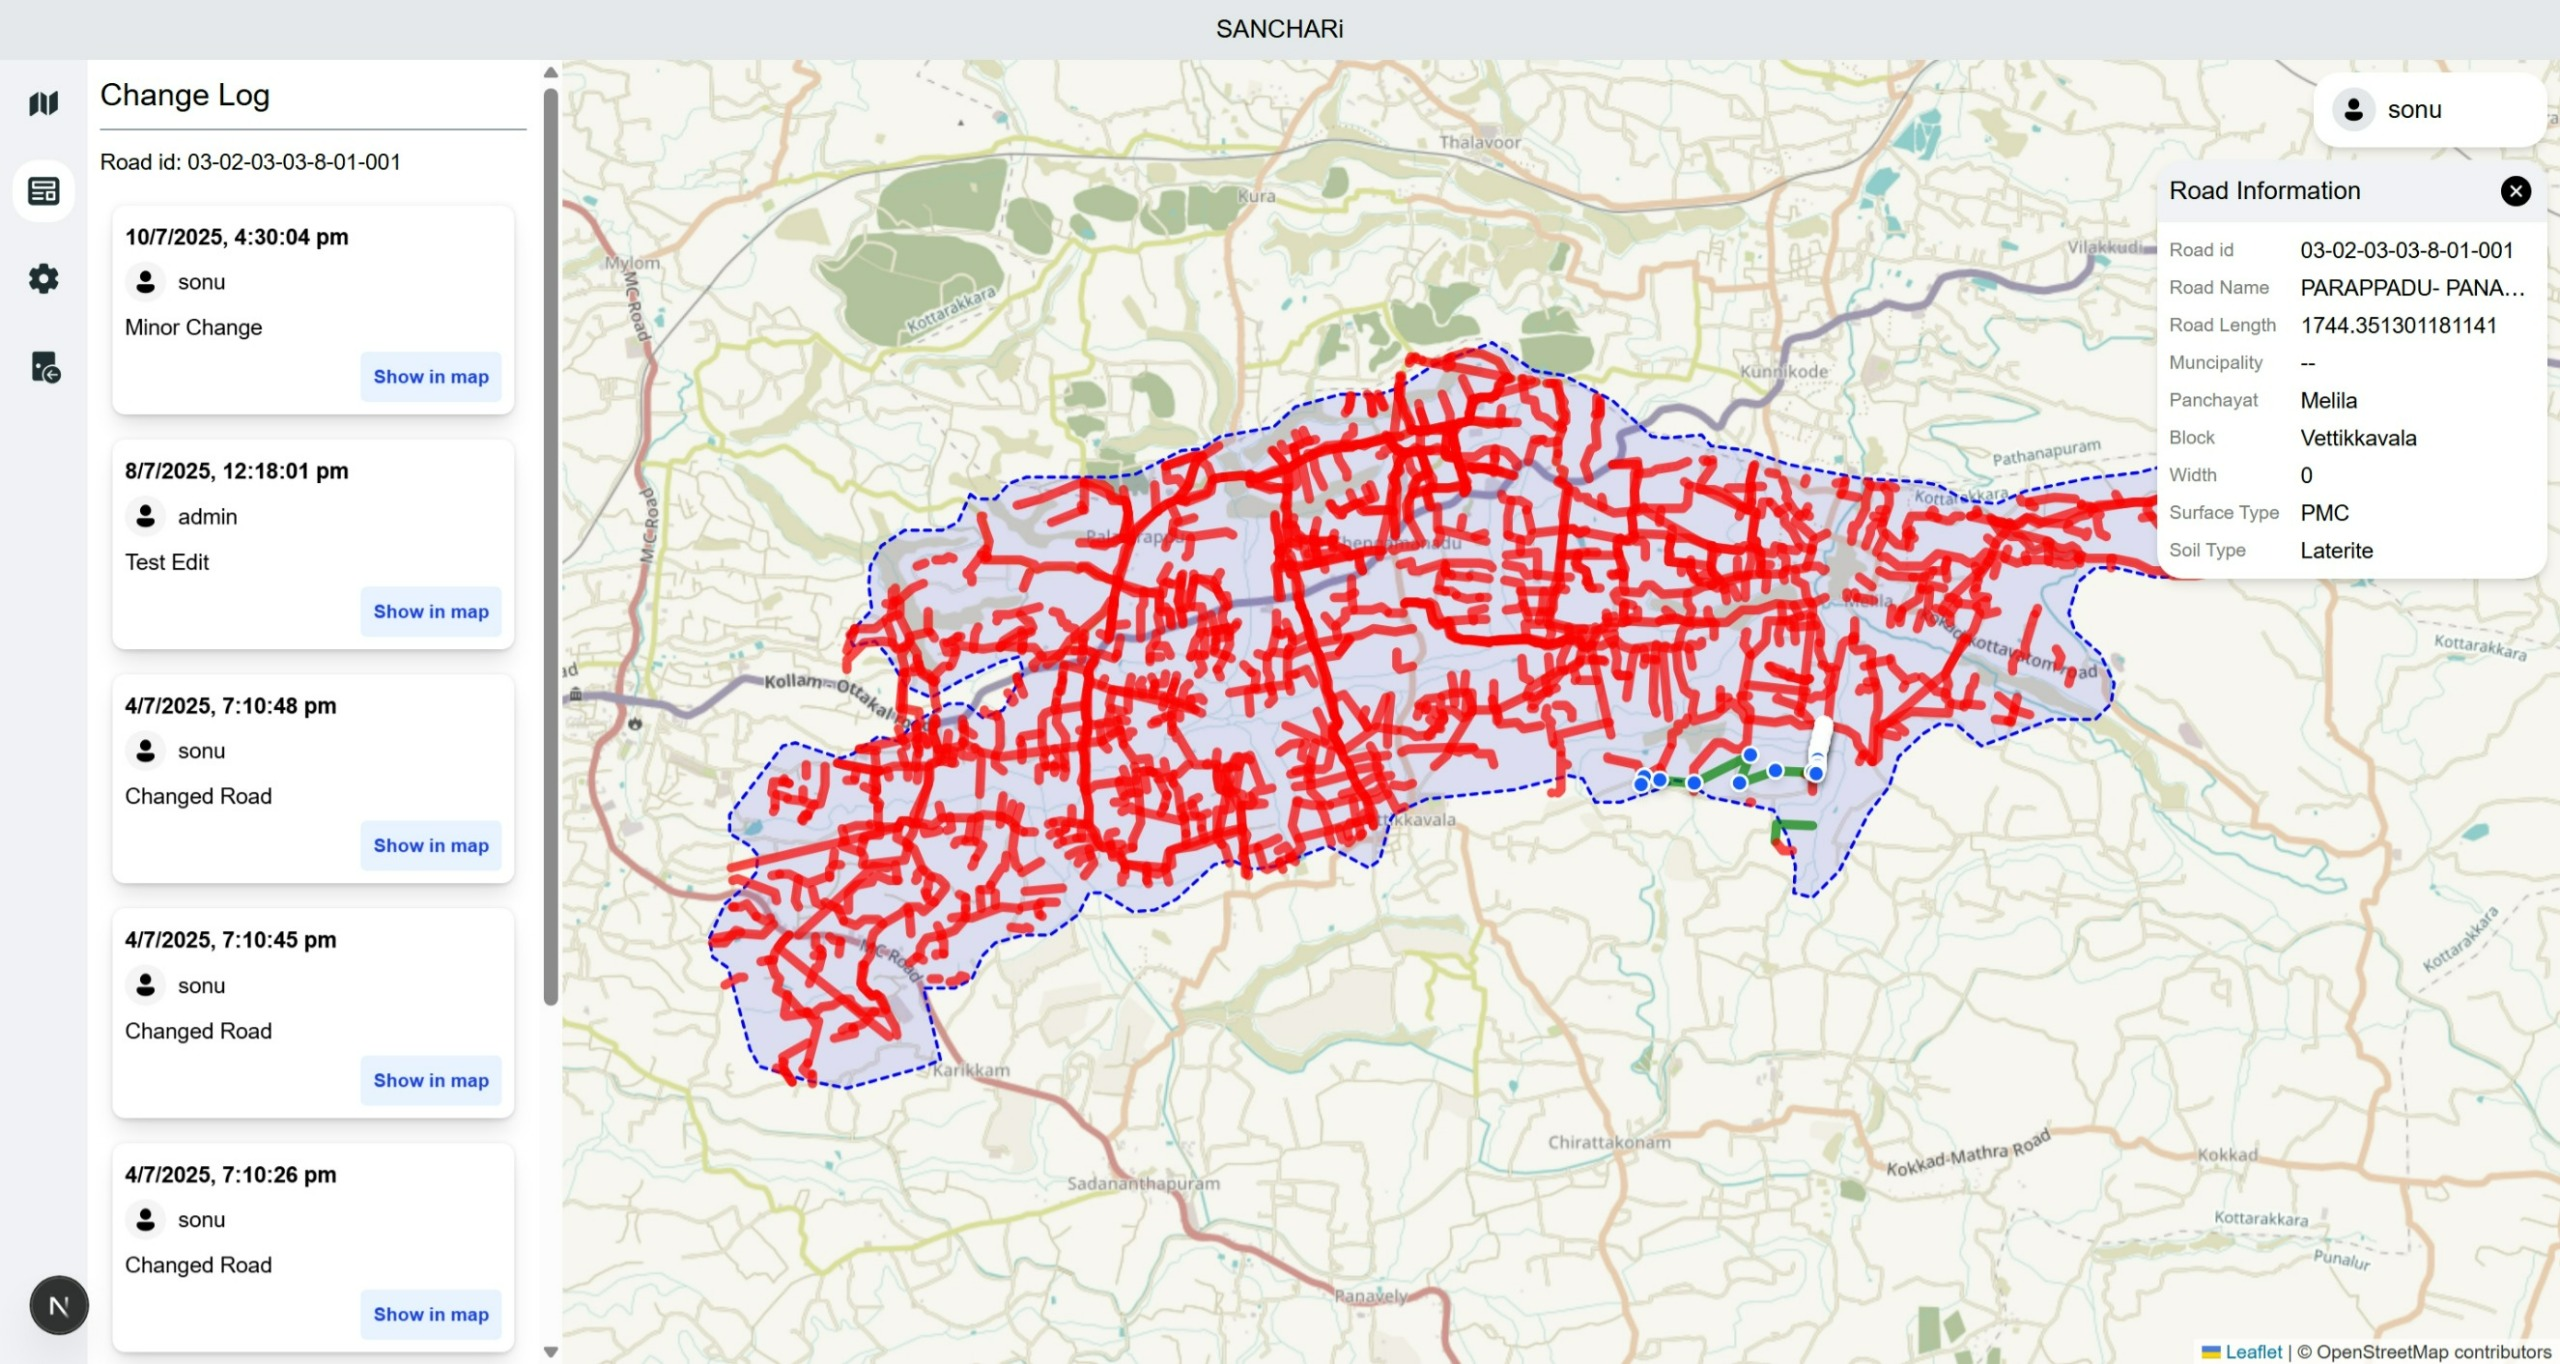
\includegraphics[width=0.9\linewidth]{changelog.jpg}}
\caption{Highlighting a selected road vector for interactive node modification. The robust PostgreSQL-backed Change Log tracks user edits and enables spatial rollbacks.}
\label{fig:changelog}
\end{figure}

The responsive Leaflet web editor enables local administrative staff to make manual improvements to the map, including connecting dangling road segments, aligning missing intersections, and adding unpaved agricultural paths. The built-in change-log feature is intended to maintain a record of edits and permit reversal of incorrect or unauthorized changes. The original draft describes these operations as an on-the-ground implementation addressing network gaps that had disrupted automated route calculations; however, no user-study logs or before-and-after routing measurements are supplied, so the present paper treats this as a system capability and case-study observation rather than a quantified result.

Figures~\ref{fig:homepage}--\ref{fig:changelog} illustrate the map landing view, editor controls, and change-log panel, respectively.

\subsection{Protocol for a Confirmatory Field Evaluation}\label{sec:field_protocol}
A confirmatory study should begin with a geographically separated set of Kerala image scenes representing vegetated rural roads, dense urban blocks, and coastal corridors. Each scene needs a date, sensor, ground sampling distance, coordinate reference system, and manually verified road reference. Source scenes, not overlapping tiles, should define the training, validation, and test partitions. A second annotator should resolve ambiguous tracks and temporary flood routes, because disagreement in the reference itself can dominate a thin-road pixel score. This design would test whether the DeepGlobe-trained model transfers across landscape and sensor changes.

For the automated stage, the same held-out scenes should be processed with and without TTA and graph cleanup, retaining both probability masks and exported GeoJSON. Report pixel IoU, precision, recall, and centerline measures under a fixed threshold-selection rule. For the network stage, compare connected components, matched intersections, and shortest-path accessibility between sampled origin-destination pairs. Report error by scene type instead of only a pooled average, because a strong urban result can conceal failures beneath canopy. The coordinate transforms and raster resolution used for every output should be logged so that a spatially displaced but visually plausible overlay is counted as an error.

For the human-in-the-loop stage, assign comparable regions to assisted and manual-only mapping workflows. Record review time, additions, deletions, undo operations, and accepted road length, then have an independent reviewer inspect the final vectors against the same ground truth. A reasonable primary outcome is valid connected road length per unit of reviewer time, with false junctions and missed segments as safety outcomes. These measurements would support a claim of operational benefit; screenshots alone cannot. No such trial is claimed here.

\section{Discussion and Socio-Technical Impact}

The utilization of this collaborative GIS platform for mapping has implications beyond the algorithmic optimization proposed by the authors. The production of authoritative map data has often been the province of state agencies or commercial entities, resulting in a top-down approach that can leave local communities unable to contribute their knowledge of the region to formal cartographic records. Such records may then be slow to reflect the immediate realities of communities.

The collaborative nature of the system, which uses the SANCHARi deep learning framework combined with a PGIS frontend, offers one way to broaden participation. Existing Volunteered Geographic Information (VGI) infrastructures require substantial time and skill from volunteer mappers. Meanwhile, a fully automated remote-sensing paradigm is inaccessible to many non-specialists and cannot reliably capture every nuance of the built environment. False predictions in early iterations of this system are especially concerning for forested rural stretches of Kerala, where the algorithm can have difficulty distinguishing vegetation, roads, and canal networks.

The system described in this paper combines automated candidate generation with locally supervised editing. By utilizing the EfficientNet-B4 network for feature detection, it aims to reduce the initial digitization burden while allowing end users to apply domain expertise to the generated vectors. Local administrators, including Panchayat members and municipal survey staff without extensive surveying experience, can participate through a focused review interface. Their local knowledge can guide adjustments such as adding roads obscured by rubber plantations and removing false positives caused by tiled roofs or seasonal flooding. The extent of any time saving remains to be measured in a controlled study.

The proposed approach is relevant to climate-related emergencies. The areas under investigation are susceptible to monsoon flooding and landslides capable of blocking last-mile connectivity. Centralized map updates may be too slow for time-sensitive response. A collaborative map could support rapid triage when suitable new imagery becomes available: the model would suggest candidate routes, and local rescue workers or administrators would review, approve, or reject them in the web interface. A suggested route must still be checked against current ground conditions before being used for navigation. This workflow is a proposed application rather than a measured disaster-response result.

The described research offers a framework for crowdsourced mapping under changing conditions. The central observation is that automated extraction and manual mapping each have limitations for sustaining up-to-date cartography. Local-government operations depend on accurate vector-based road layers, whose creation requires time and expertise. The proposed solution retains authoritative supervision while using an automated pipeline to reduce routine vectorization. It connects computer vision with civic participation and provides a design for continuous topographic audits, subject to the field evaluation described above.

\subsection{Limits of the Present Evidence}
The approximate IoU values summarize project development but lack a common published test protocol, per-scene results, and uncertainty estimates. The current train-validation partition is made after overlapping tiling, which risks spatial leakage between neighboring patches. The reported score therefore describes an internal tile split and should not be generalized to Kerala imagery or post-disaster scenes. Moreover, graph cleanup occurs after probability-map validation; an 80\% pixel score does not measure topological correctness of the exported lines.

The guide's model implementation and the draft's collaborative WebGIS are documented at different levels of detail. The Python repository supports inspection of training, inference, and GeoJSON conversion, while the provided paper and screenshots describe the editor and transaction workflow. Without a linked deployment record, transaction logs, or a controlled user study, claims about editor throughput, permanent auditability, and real-time conflict handling remain design claims. The difference does not remove the usefulness of the architecture; it defines the next evidence needed before operational adoption.

Finally, image recency, canopy, water, shadows, and changes in ground resolution can all alter the reliability of a candidate road. Automatic gap closing can create false connections, and simplification can remove meaningful short segments. For emergency use, local review should remain mandatory before a suggested route is treated as passable. A future release should add uncertainty cues to each candidate, preserve model and imagery provenance in the database, and evaluate independent Kerala scenes and reviewer decisions with a preregistered protocol.

\section{Conclusion}
This study presents a human-in-the-loop framework that integrates deep-learning-based road extraction with collaborative editing of maps. Upgrading the network backbone to EfficientNet-B4 and using Combo Loss with optional hard-example and Lov\'{a}sz fine-tuning led to a project-reported validation IoU of approximately 80\% on DeepGlobe tiles. Pairing the model with a responsive front end implemented in Next.js and Leaflet with PostGIS support gives reviewers a way to correct errors caused by complex terrain. Independent scene-level validation in Kerala and a measured editor study are the next steps before claiming an operational improvement. 

\begin{thebibliography}{16}
\bibitem{b1} Jing, C., Zhu, Y., Fu, J., Dong, M.: A lightweight collaborative GIS data editing approach to support urban planning. \emph{Sustainability} \textbf{11}(16), 4437 (2019). \url{https://doi.org/10.3390/su11164437}
\bibitem{b2} Butt, M.A., Mahmood, S.A., Raza, S.M.H.: GeoWebEX: an open-source online system for synchronous collaboration on geographic information. \emph{Applied Geomatics} \textbf{10}, 123--145 (2018). \url{https://doi.org/10.1007/s12518-018-0204-8}
\bibitem{b3} Kantartzis, A., Malesios, C.: A decision support system web-application for the management of forest road network. \emph{Journal of Environmental Science and Engineering A}, 8--21 (2018). \url{https://doi.org/10.17265/2162-5298/2018.01.002}
\bibitem{b4} Netek, R., Pohankova, T., Bittner, O., Urban, D.: Geospatial analysis in web browsers: comparison study on WebGIS process-based applications. \emph{ISPRS International Journal of Geo-Information} \textbf{12}(9), 374 (2023). \url{https://doi.org/10.3390/ijgi12090374}
\bibitem{b5} Pollino, M., Fattoruso, G., La Porta, L., Della Rocca, A.B., James, V.: Collaborative open source geospatial tools and maps supporting the response planning to disastrous earthquake events. \emph{Future Internet} \textbf{4}, 451--468 (2012). \url{https://doi.org/10.3390/fi4020451}
\bibitem{b6} Bastani, F., He, S., Abbar, S., Alizadeh, M., Balakrishnan, H., Chawla, S., Madden, S.: Machine-assisted map editing. In: \emph{26th ACM SIGSPATIAL International Conference on Advances in Geographic Information Systems}, pp. 23--32 (2018). \url{https://doi.org/10.1145/3274895.3274927}
\bibitem{b7} Stoven-Dubois, A., Kiala Miguel, K., Dziri, A., Leroy, B., Chapuis, R.: A collaborative framework for high-definition mapping. In: \emph{2019 IEEE Intelligent Transportation Systems Conference (ITSC)} (2019).
\bibitem{b8} Shi, Q., Liu, X., Li, X.: Road detection from remote sensing images by generative adversarial networks. \emph{IEEE Access} \textbf{6}, 25486--25494 (2018). \url{https://doi.org/10.1109/ACCESS.2017.2773142}
\bibitem{b9} Bastani, F., He, S., Abbar, S., Alizadeh, M., Balakrishnan, H., Chawla, S., Madden, S., DeWitt, D.: RoadTracer: automatic extraction of road networks from aerial images. In: \emph{Proceedings of the IEEE Conference on Computer Vision and Pattern Recognition}, pp. 4720--4728 (2018).
\bibitem{b10} He, S., Bastani, F., Jagwani, S., Alizadeh, M., Balakrishnan, H., Chawla, S., Elshrif, M.M., Madden, S., Sadeghi, M.A.: Sat2Graph: road graph extraction through graph-tensor encoding. In: \emph{European Conference on Computer Vision} (2020). \url{https://doi.org/10.1007/978-3-030-58586-0_4}
\bibitem{b11} Ronneberger, O., Fischer, P., Brox, T.: U-Net: convolutional networks for biomedical image segmentation. In: \emph{Medical Image Computing and Computer-Assisted Intervention} (2015). \url{https://doi.org/10.1007/978-3-319-24574-4_28}
\bibitem{b12} He, K., Zhang, X., Ren, S., Sun, J.: Deep residual learning for image recognition. In: \emph{Proceedings of the IEEE Conference on Computer Vision and Pattern Recognition}, pp. 770--778 (2016).
\bibitem{b13} Zhou, Z., Siddiquee, M.M.R., Tajbakhsh, N., Liang, J.: UNet++: a nested U-Net architecture for medical image segmentation. In: \emph{Deep Learning in Medical Image Analysis and Multimodal Learning for Clinical Decision Support}, pp. 3--11 (2018). \url{https://doi.org/10.1007/978-3-030-00889-5_1}
\bibitem{b14} Tan, M., Le, Q.V.: EfficientNet: rethinking model scaling for convolutional neural networks. In: \emph{Proceedings of the 36th International Conference on Machine Learning}, PMLR \textbf{97}, 6105--6114 (2019).
\bibitem{b15} Berman, M., Rannen Triki, A., Blaschko, M.B.: The Lov\'{a}sz-Softmax loss: a tractable surrogate for the optimization of the intersection-over-union measure in neural networks. In: \emph{Proceedings of the IEEE Conference on Computer Vision and Pattern Recognition}, pp. 4413--4421 (2018).
\bibitem{b16} Demir, I., Koperski, K., Lindenbaum, D., Pang, G., Huang, J., Basu, S., Hughes, F., Tuia, D., Raskar, R.: DeepGlobe 2018: a challenge to parse the Earth through satellite images. In: \emph{Proceedings of the IEEE Conference on Computer Vision and Pattern Recognition Workshops}, pp. 172--181 (2018).
\end{thebibliography}

\end{document}
